 
%% bare_conf.tex
%% V1.4b
%% 2015/08/26
%% by Michael Shell
%% See:
%% http://www.michaelshell.org/
%% for current contact information.
%%
%% This is a skeleton file demonstrating the use of IEEEtran.cls
%% (requires IEEEtran.cls version 1.8b or later) with an IEEE
%% conference paper.
%%
%% Support sites:
%% http://www.michaelshell.org/tex/ieeetran/
%% http://www.ctan.org/pkg/ieeetran
%% and
%% http://www.ieee.org/

%%*************************************************************************
%% Legal Notice:
%% This code is offered as-is without any warranty either expressed or
%% implied; without even the implied warranty of MERCHANTABILITY or
%% FITNESS FOR A PARTICULAR PURPOSE! 
%% User assumes all risk.
%% In no event shall the IEEE or any contributor to this code be liable for
%% any damages or losses, including, but not limited to, incidental,
%% consequential, or any other damages, resulting from the use or misuse
%% of any information contained here.
%%
%% All comments are the opinions of their respective authors and are not
%% necessarily endorsed by the IEEE.
%%
%% This work is distributed under the LaTeX Project Public License (LPPL)
%% ( http://www.latex-project.org/ ) version 1.3, and may be freely used,
%% distributed and modified. A copy of the LPPL, version 1.3, is included
%% in the base LaTeX documentation of all distributions of LaTeX released
%% 2003/12/01 or later.
%% Retain all contribution notices and credits.
%% ** Modified files should be clearly indicated as such, including  **
%% ** renaming them and changing author support contact information. **
%%*************************************************************************


% *** Authors should verify (and, if needed, correct) their LaTeX system  ***
% *** with the testflow diagnostic prior to trusting their LaTeX platform ***
% *** with production work. The IEEE's font choices and paper sizes can   ***
% *** trigger bugs that do not appear when using other class files.       ***                          ***
% The testflow support page is at:
% http://www.michaelshell.org/tex/testflow/



\documentclass[conference, a4paper]{IEEEtran}
% Some Computer Society conferences also require the compsoc mode option,
% but others use the standard conference format.
%
% If IEEEtran.cls has not been installed into the LaTeX system files,
% manually specify the path to it like:
% \documentclass[conference]{../sty/IEEEtran}





% Some very useful LaTeX packages include:
% (uncomment the ones you want to load)


% *** MISC UTILITY PACKAGES ***
%
%\usepackage{ifpdf}
% Heiko Oberdiek's ifpdf.sty is very useful if you need conditional
% compilation based on whether the output is pdf or dvi.
% usage:
% \ifpdf
%   % pdf code
% \else
%   % dvi code
% \fi
% The latest version of ifpdf.sty can be obtained from:
% http://www.ctan.org/pkg/ifpdf
% Also, note that IEEEtran.cls V1.7 and later provides a builtin
% \ifCLASSINFOpdf conditional that works the same way.
% When switching from latex to pdflatex and vice-versa, the compiler may
% have to be run twice to clear warning/error messages.






% *** CITATION PACKAGES ***
%
\usepackage{cite}
% cite.sty was written by Donald Arseneau
% V1.6 and later of IEEEtran pre-defines the format of the cite.sty package
% \cite{} output to follow that of the IEEE. Loading the cite package will
% result in citation numbers being automatically sorted and properly
% "compressed/ranged". e.g., [1], [9], [2], [7], [5], [6] without using
% cite.sty will become [1], [2], [5]--[7], [9] using cite.sty. cite.sty's
% \cite will automatically add leading space, if needed. Use cite.sty's
% noadjust option (cite.sty V3.8 and later) if you want to turn this off
% such as if a citation ever needs to be enclosed in parenthesis.
% cite.sty is already installed on most LaTeX systems. Be sure and use
% version 5.0 (2009-03-20) and later if using hyperref.sty.
% The latest version can be obtained at:
% http://www.ctan.org/pkg/cite
% The documentation is contained in the cite.sty file itself.






% *** GRAPHICS RELATED PACKAGES ***
%
\ifCLASSINFOpdf
  \usepackage[pdftex]{graphicx}
  % declare the path(s) where your graphic files are
  % \graphicspath{{../pdf/}{../jpeg/}}
  % and their extensions so you won't have to specify these with
  % every instance of \includegraphics
  % \DeclareGraphicsExtensions{.pdf,.jpeg,.png}
\else
  % or other class option (dvipsone, dvipdf, if not using dvips). graphicx
  % will default to the driver specified in the system graphics.cfg if no
  % driver is specified.
  % \usepackage[dvips]{graphicx}
  % declare the path(s) where your graphic files are
  % \graphicspath{{../eps/}}
  % and their extensions so you won't have to specify these with
  % every instance of \includegraphics
  % \DeclareGraphicsExtensions{.eps}
\fi
% graphicx was written by David Carlisle and Sebastian Rahtz. It is
% required if you want graphics, photos, etc. graphicx.sty is already
% installed on most LaTeX systems. The latest version and documentation
% can be obtained at: 
% http://www.ctan.org/pkg/graphicx
% Another good source of documentation is "Using Imported Graphics in
% LaTeX2e" by Keith Reckdahl which can be found at:
% http://www.ctan.org/pkg/epslatex
%
% latex, and pdflatex in dvi mode, support graphics in encapsulated
% postscript (.eps) format. pdflatex in pdf mode supports graphics
% in .pdf, .jpeg, .png and .mps (metapost) formats. Users should ensure
% that all non-photo figures use a vector format (.eps, .pdf, .mps) and
% not a bitmapped formats (.jpeg, .png). The IEEE frowns on bitmapped formats
% which can result in "jaggedy"/blurry rendering of lines and letters as
% well as large increases in file sizes.
%
% You can find documentation about the pdfTeX application at:
% http://www.tug.org/applications/pdftex





% *** MATH PACKAGES ***
%
\usepackage{amsmath}
% A popular package from the American Mathematical Society that provides
% many useful and powerful commands for dealing with mathematics.
%
% Note that the amsmath package sets \interdisplaylinepenalty to 10000
% thus preventing page breaks from occurring within multiline equations. Use:
%\interdisplaylinepenalty=2500
% after loading amsmath to restore such page breaks as IEEEtran.cls normally
% does. amsmath.sty is already installed on most LaTeX systems. The latest
% version and documentation can be obtained at:
% http://www.ctan.org/pkg/amsmath


\usepackage{color}


% *** SPECIALIZED LIST PACKAGES ***
%
\usepackage{algorithmic}
% algorithmic.sty was written by Peter Williams and Rogerio Brito.
% This package provides an algorithmic environment fo describing algorithms.
% You can use the algorithmic environment in-text or within a figure
% environment to provide for a floating algorithm. Do NOT use the algorithm
% floating environment provided by algorithm.sty (by the same authors) or
% algorithm2e.sty (by Christophe Fiorio) as the IEEE does not use dedicated
% algorithm float types and packages that provide these will not provide
% correct IEEE style captions. The latest version and documentation of
% algorithmic.sty can be obtained at:
% http://www.ctan.org/pkg/algorithms
% Also of interest may be the (relatively newer and more customizable)
% algorithmicx.sty package by Szasz Janos:
% http://www.ctan.org/pkg/algorithmicx




% *** ALIGNMENT PACKAGES ***
%
\usepackage{array}
% Frank Mittelbach's and David Carlisle's array.sty patches and improves
% the standard LaTeX2e array and tabular environments to provide better
% appearance and additional user controls. As the default LaTeX2e table
% generation code is lacking to the point of almost being broken with
% respect to the quality of the end results, all users are strongly
% advised to use an enhanced (at the very least that provided by array.sty)
% set of table tools. array.sty is already installed on most systems. The
% latest version and documentation can be obtained at:
% http://www.ctan.org/pkg/array


% IEEEtran contains the IEEEeqnarray family of commands that can be used to
% generate multiline equations as well as matrices, tables, etc., of high
% quality.




% *** SUBFIGURE PACKAGES ***
%\ifCLASSOPTIONcompsoc
%  \usepackage[caption=false,font=normalsize,labelfont=sf,textfont=sf]{subfig}
%\else
  \usepackage[caption=false,font=footnotesize]{subfig}
%\fi
% subfig.sty, written by Steven Douglas Cochran, is the modern replacement
% for subfigure.sty, the latter of which is no longer maintained and is
% incompatible with some LaTeX packages including fixltx2e. However,
% subfig.sty requires and automatically loads Axel Sommerfeldt's caption.sty
% which will override IEEEtran.cls' handling of captions and this will result
% in non-IEEE style figure/table captions. To prevent this problem, be sure
% and invoke subfig.sty's "caption=false" package option (available since
% subfig.sty version 1.3, 2005/06/28) as this is will preserve IEEEtran.cls
% handling of captions.
% Note that the Computer Society format requires a larger sans serif font
% than the serif footnote size font used in traditional IEEE formatting
% and thus the need to invoke different subfig.sty package options depending
% on whether compsoc mode has been enabled.
%
% The latest version and documentation of subfig.sty can be obtained at:
% http://www.ctan.org/pkg/subfig


\usepackage{tikz}
% *** FLOAT PACKAGES ***
%
%\usepackage{fixltx2e}
% fixltx2e, the successor to the earlier fix2col.sty, was written by
% Frank Mittelbach and David Carlisle. This package corrects a few problems
% in the LaTeX2e kernel, the most notable of which is that in current
% LaTeX2e releases, the ordering of single and double column floats is not
% guaranteed to be preserved. Thus, an unpatched LaTeX2e can allow a
% single column figure to be placed prior to an earlier double column
% figure.
% Be aware that LaTeX2e kernels dated 2015 and later have fixltx2e.sty's
% corrections already built into the system in which case a warning will
% be issued if an attempt is made to load fixltx2e.sty as it is no longer
% needed.
% The latest version and documentation can be found at:
% http://www.ctan.org/pkg/fixltx2e


%\usepackage{stfloats}
% stfloats.sty was written by Sigitas Tolusis. This package gives LaTeX2e
% the ability to do double column floats at the bottom of the page as well
% as the top. (e.g., "\begin{figure*}[!b]" is not normally possible in
% LaTeX2e). It also provides a command:
%\fnbelowfloat
% to enable the placement of footnotes below bottom floats (the standard
% LaTeX2e kernel puts them above bottom floats). This is an invasive package
% which rewrites many portions of the LaTeX2e float routines. It may not work
% with other packages that modify the LaTeX2e float routines. The latest
% version and documentation can be obtained at:
% http://www.ctan.org/pkg/stfloats
% Do not use the stfloats baselinefloat ability as the IEEE does not allow
% \baselineskip to stretch. Authors submitting work to the IEEE should note
% that the IEEE rarely uses double column equations and that authors should try
% to avoid such use. Do not be tempted to use the cuted.sty or midfloat.sty
% packages (also by Sigitas Tolusis) as the IEEE does not format its papers in
% such ways.
% Do not attempt to use stfloats with fixltx2e as they are incompatible.
% Instead, use Morten Hogholm'a dblfloatfix which combines the features
% of both fixltx2e and stfloats:
%
% \usepackage{dblfloatfix}
% The latest version can be found at:
% http://www.ctan.org/pkg/dblfloatfix




% *** PDF, URL AND HYPERLINK PACKAGES ***
%
%\usepackage{url}
% url.sty was written by Donald Arseneau. It provides better support for
% handling and breaking URLs. url.sty is already installed on most LaTeX
% systems. The latest version and documentation can be obtained at:
% http://www.ctan.org/pkg/url
% Basically, \url{my_url_here}.




% *** Do not adjust lengths that control margins, column widths, etc. ***
% *** Do not use packages that alter fonts (such as pslatex).         ***
% There should be no need to do such things with IEEEtran.cls V1.6 and later.
% (Unless specifically asked to do so by the journal or conference you plan
% to submit to, of course. )


% MP: nice rules in tables
\usepackage{booktabs}

%% ridurre spazio formule
\setlength{\abovedisplayskip}{0.14cm}
\setlength{\belowdisplayskip}{0.14cm}

%% ridurre spazio figure
\usepackage{caption}
%\usepackage{subcaption}
\captionsetup[figure]{skip=2pt,font=footnotesize}
\setlength{\belowcaptionskip}{-12pt}
\setlength{\skip\footins}{0.3cm}
\linespread{.94}

% correct bad hyphenation here
\hyphenation{op-tical net-works semi-conduc-tor}


\begin{document}

%
% paper title
% Titles are generally capitalized except for words such as a, an, and, as,
% at, but, by, for, in, nor, of, on, or, the, to and up, which are usually
% not capitalized unless they are the first or last word of the title.
% Linebreaks \\ can be used within to get better formatting as desired.
% Do not put math or special symbols in the title.
\title{Learning methods for long-term channel gain prediction in wireless networks}


% author names and affiliations
% use a multiple column layout for up to three different
% affiliations
\author{\IEEEauthorblockN{Federico Chiariotti,
Davide Del Testa,
Michele Polese,\\
Andrea Zanella,
Giorgio Maria Di Nunzio,
and Michele Zorzi}
\IEEEauthorblockA{Department of Information Engineering (DEI), University of Padua, Italy\\
Email: \{chiariot, deltesta, polesemi, zanella, dinunzio, zorzi\}@dei.unipd.it}}

% conference papers do not typically use \thanks and this command
% is locked out in conference mode. If really needed, such as for
% the acknowledgment of grants, issue a \IEEEoverridecommandlockouts
% after \documentclass

% for over three affiliations, or if they all won't fit within the width
% of the page, use this alternative format:
% 
%\author{\IEEEauthorblockN{Michael Shell\IEEEauthorrefmark{1},
%Homer Simpson\IEEEauthorrefmark{2},
%James Kirk\IEEEauthorrefmark{3}, 
%Montgomery Scott\IEEEauthorrefmark{3} and
%Eldon Tyrell\IEEEauthorrefmark{4}}
%\IEEEauthorblockA{\IEEEauthorrefmark{1}School of Electrical and Computer Engineering\\
%Georgia Institute of Technology,
%Atlanta, Georgia 30332--0250\\ Email: see http://www.michaelshell.org/contact.html}
%\IEEEauthorblockA{\IEEEauthorrefmark{2}Twentieth Century Fox, Springfield, USA\\
%Email: homer@thesimpsons.com}
%\IEEEauthorblockA{\IEEEauthorrefmark{3}Starfleet Academy, San Francisco, California 96678-2391\\
%Telephone: (800) 555--1212, Fax: (888) 555--1212}
%\IEEEauthorblockA{\IEEEauthorrefmark{4}Tyrell Inc., 123 Replicant Street, Los Angeles, California 90210--4321}}




% use for special paper notices
%\IEEEspecialpapernotice{(Invited Paper)}




% make the title area
\maketitle

% As a general rule, do not put math, special symbols or citations
% in the abstract
\begin{abstract}
Efficiently allocating resources and predicting cell handovers is essential in modern wireless networks; however, this is only possible if there is an efficient way to estimate the future state of the network.
In order to accomplish this, we investigate two learning techniques to predict the long-term channel gains in a wireless network. Previous works in the literature found efficient methods to perform this prediction with the aid of a GPS signal: in this work, we predict the future channel gains using only past channel samples, without any geographical information.
\end{abstract}

% no keywords




% For peer review papers, you can put extra information on the cover
% page as needed:
% \ifCLASSOPTIONpeerreview
% \begin{center} \bfseries EDICS Category: 3-BBND \end{center}
% \fi
%
% For peerreview papers, this IEEEtran command inserts a page break and
% creates the second title. It will be ignored for other modes.
\IEEEpeerreviewmaketitle



\section{Introduction}
Global mobile data traffic has grown 4,000-fold over the past 10 years \cite{cisco2016global}, and its growth is expected to continue, fueled by the high bandwidth demands of multimedia applications (video alone already accounted for a majority of the total mobile data traffic in 2015).

As mobile multimedia applications have strict Quality of Service (QoS) requirements, the development of optimal resource allocation techniques is a priority for both industry and academia. Applications such as video streaming would greatly benefit from an accurate channel prediction, and prediction-based adaptive streaming systems have already been proposed \cite{mekki2015anticipatory}. Most of the efforts in channel prediction have focused on Multiple Input Multiple Output (MIMO) techniques on short time horizons, but several works \cite{zhou2004accurate} \cite{liao2015channel} have expressed the need for long-term accurate channel gain predictions. 

In this paper, we investigate learning methods to predict the wireless channel gain on a long-term scale, without any inputs other than the time-averaged Received Signal Strength Indicator (RSSI). This prediction is performed by the Base Station (BS), which is the only fixed element in the network; the BS can indirectly learn the mobility patterns of the mobile users and the fading characteristics of the channel by observing patterns in their RSSI.

The two machine learning techniques we use are Graphical Bayesian (GB) models and Support Vector Regression machines (SVRs). The GB model can be used as a baseline, as it does not try to generalize its experience, but simply considers each class as a separate classification problem. SVRs are able to find and generalize patterns in the data, making better predictions with fewer data.

The rest of this work is organized as follows: Section II presents the state of the art in channel prediction, and Section III illustrates the learning techniques we used. Section IV presents the model we used to generate the data and the simulation results we obtained, and Section V concludes the paper.

\section{State of the art}

Wireless links are often modeled as Rayleigh fading channels. Most model-based prediction systems concentrate on short-term predictions of the fading envelope for wideband channels~\cite{dong2001prediction}, and cannot be directly used for optimization at the higher layers. As mobility was not a central issue, the relatively predictable nature of path loss made long-range channel prediction an easy problem.

Shen \emph{et al.} predict future channel quality from receiver-side Channel State Information (CSI) \cite{shen2003short}, but the Autoregressive (AR) filters they use are only accurate on a timescale of a few milliseconds. The work in \cite{wong2004long} proposes an OFDM-specific prediction method based on time-domain statistics with a slightly longer range, but the timescales for accurate predictions are still far below $100$ ms.

Another AR model is proposed by Jarinova \cite{jarinova2013autoregressive}, but its predictions are extremely short-range and how to choose the order of the filter is an issue.

Several works in the literature have attempted to solve the long-term channel prediction problem with machine learning techniques. A typical example is Ramanan and Walsh's channel prediction algorithm for sensor networks~\cite{ramanan2010distributed}. It is a distributed algorithm that employs message passing techniques to minimize the Kullback-Leibler divergence between the expected prior distribution and the actual posterior.

The problem of channel prediction is central in Cognitive Radio (CR) systems, and Demestichas \emph{et al.} propose a Bayesian Network (BN) \cite{demestichas2009enhancing} to solve this issue. Their BN predicts the future capacity for each possible CR configuration, and adapts to channel conditions online, but it is meant for Modulation and Coding System (MCS) selection rather than for optimization at higher layers.

Flushing \emph{et al.} take an empirical approach \cite{flushing2012mobility}, combining a probing mechanism with Support Vector Regression (SVR) to predict link quality in dense wireless networks. Thanks to mobility, the probing system can learn about several different topologies and extend this knowledge to larger, denser networks.

Finally, Liao \emph{et al.} perform long-term channel prediction \cite{liao2015channel} using both spatial and temporal information. The authors propose a Gaussian Process (GP) regression, training the system through a series of routes on a city map. Their prediction method is robust against spatial errors, with better performance than both Support Vector Machines (SVMs) and AR filters. Although their method is sound for large-scale scenarios, it does not deal with smaller cells and needs Global Positioning System (GPS) information from clients, which might not be available.

\section{Learning techniques}

The two learning techniques we used are extremely versatile: they do not assume a specific channel model, so they can be trained and deployed on any wireless channel with only minor adjustments. In order to make the necessary data easy to obtain in a practical scenario, we decided to use the Received Signal Strength Indicator (RSSI) \cite{wu2008study} as training data, averaging the data over a long enough window to reduce measurement error and avoid holes in the sampling even in a congested network.


\subsection{Graphical Bayesian Model}

The GB model can be represented by the graph shown in Fig.~\ref{fig:graphical_bayes}. As the Bayesian model only works for discrete attributes, the dynamic interval of the channel gain needs to be discretized into $M$ classes. The memory-$n$ Bayesian model uses the past $n$ samples as features, resulting in $M^n$ possible combinations. The predictor is essentially a classifier, in which the future  channel sample is the correct class.

The multimodal classifier is implemented by a Dirichlet distribution \cite{geiger1995characterization} over the $M$-dimensional simplex, which is parameterized by a real non-negative vector $\alpha$:

\begin{align}
 p(X=(x_1,\dots,x_M)|\alpha)&=\frac{1}{B(\alpha)}\prod_{i=1}^M x_i^{\alpha_i-1},
\end{align}
where the normalizing constant $B(\alpha)$ is the multivariate Beta function \cite{NIST:DLMF}. The random vector $X=(X_1,\dots,X_M)$ is a probability distribution over the $M$ classes, representing the probability that the given sample is in each class (i.e., the probability distribution of the next channel sample). The expected value of $X$ is given by:
\begin{align}
 \text{E}[X_i]&=\frac{\alpha_i}{\sum_{j=1}^M \alpha_j}\\
 \text{Var}[X_i]&=\frac{\alpha_i\sum_{j\neq i} \alpha_j}{(\sum_{j=1}^M \alpha_j)^2(\sum_{j=1}^M \alpha_j+1)}
\end{align}

Intuitively, the value of $\alpha_i$ relative to the sum of the $\alpha$ vector is a measure of how probable a class is, and the value of the sum measures the uncertainty on that probability. The conjugate distribution of the Dirichlet distribution is the Dirichlet-multinomial distribution; Bayesian inference can be performed by generating a new parameter vector $\alpha'$, defined as
\begin{align}
 \alpha'_i&=\alpha_i+n_i,
\end{align}
where $n_i$ is the number of observed transitions to class $i$. The prediction can be performed by taking the expected probability distribution of the next sample, given by
\begin{align}
 p(i)&=\frac{\alpha'_i}{\sum_{j=1}^M \alpha'_j}
\end{align}
The predicted class then corresponds to the maximum probability value.

\begin{figure}[!t]
\centering
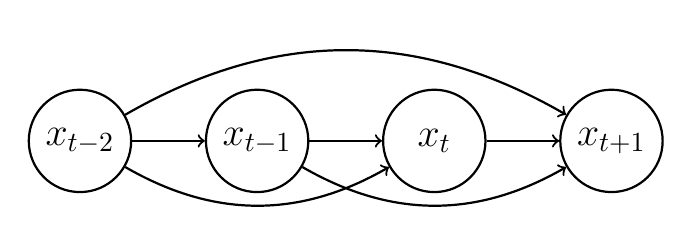
\begin{tikzpicture}[->,auto,node distance=2.25cm,
  thick,main node/.style={circle,minimum size=1.3cm,draw,font=\sffamily\Large}]

  \node[main node] (1) {$x_{t-2}$};
  \node[main node] (2) [right of=1] {$x_{t-1}$};
  \node[main node] (3) [right of=2] {$x_t$};
  \node[main node] (4) [right of=3] {$x_{t+1}$};

  \path[every node/.style={font=\sffamily\small}]
    (1) edge node [right] {} (2)
    (2) edge node [right] {} (3)
    (3) edge node [right] {} (4)
    (1) edge[bend right] node [left] {} (3)
    (2) edge[bend right] node [left] {} (4)
    (1) edge[bend left] node [left] {} (4);
    \end{tikzpicture}
\caption{Representation of the graphical Bayesian model with 3-state memory.}
\label{fig:graphical_bayes}
\end{figure}

\subsection{Support Vector Regression Machine}
Support Vector Regression (SVR) machines \cite{Vapnik1995, Drucker1997}, minimize the following cost function:
\begin{align}\label{eq:SVR_firstCost}
C \sum_i E_\epsilon(f_{\mathbf{w}}(\mathbf{x}^{(i)})-x_{t+1}^{(i)}) + \frac{1}{2} ||\mathbf{w}||^2.
\end{align}
In \eqref{eq:SVR_firstCost}, $f_{\mathbf{w}}$ is a function taking as input a memory-$n$ feature vector $\mathbf{x}^{(i)} = \left(x_{t-n+1}, \dots, x_t \right)$ and predicting a future sample $\hat x_{t+1}$, for a given training example $i$. The error between this predicted sample and the actual sample at time $t+1$, $x_{t+1}$, is then fed to an $\epsilon$-insensitive error function 
\begin{align}
E_\epsilon(z) = 
\begin{cases}
|z|-\epsilon  \hspace{0.5cm} \text{if} \quad |z| > \epsilon \\
0 \hspace{1.3cm} \text{otherwise}
\end{cases}
\end{align}
so that $f_{\mathbf{w}}$ is constrained to have maximum absolute prediction error lower than a given constant $\epsilon$ for all the training data. The second term in \eqref{eq:SVR_firstCost} accounts for regularization: the trade-off between the minimization of the two terms is governed by the constant $C$ (the reader can refer to \cite{Smola2004,Cortes1995} for more details).
\begin{figure}[!ht]
	\centering
	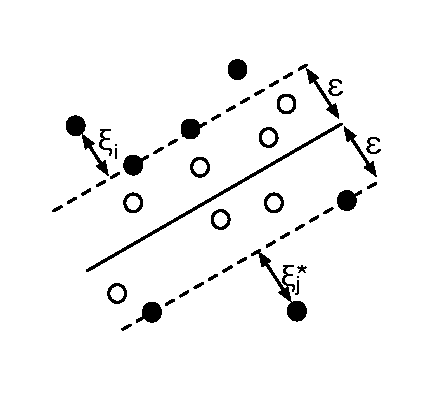
\includegraphics[width=2.5in]{./graphics/SVR.eps}
	\caption{Graphical representation of an $\epsilon$-tube with slack variables.}
	\label{fig:svr}
\end{figure}
In \eqref{eq:SVR_firstCost}, all the training examples are assumed to lie in an  ``$\epsilon$-tube'' (see \figurename~\ref{fig:svr}). However, this is not verified in general, and \eqref{eq:SVR_firstCost} can be modified so as to allow for some tolerance in the prediction errors.
Therefore, for each training example $\mathbf{x}^{(i)}$, it is possible to introduce \textit{slack variables} $\xi_i$ and $\xi_i^*$, where $\xi_i>0$ is related to a point for which $(x_{t+1}^{(i)}-f_{\mathbf{w}}(\mathbf{x}^{(i)})) > \epsilon$, and $\xi_i^*>0$ is related to a point for which $(f_{\mathbf{w}}(\mathbf{x}^{(i)})-x_{t+1}^{(i)}) < -\epsilon$. 
Training examples are thus allowed to lie outside the $\epsilon$-tube, as in \figurename~\ref{fig:svr}, provided that the corresponding slack variables are positive: this condition can be formulated as
\begin{align}
-\epsilon - \xi_i^*\leq x_{t+1}^{(i)}-f_{\mathbf{w}}(\mathbf{x}^{(i)}) & \leq +\epsilon + \xi_i \label{eq:SVR_tube1}
\end{align}
The optimization problem becomes
\begin{equation}\label{eq:SVR_secondCost}
\min C \sum_i \left(\xi_i+\xi_i^* \right) + \frac{1}{2} ||\mathbf{w}||^2,
\end{equation}
subject to the constraints $\xi_i, \xi_i^* \ge 0$, and \eqref{eq:SVR_tube1}. It can be seen that  only the examples outside
the $\epsilon$-tube contribute to the cost, with deviations being linearly penalized. Computing the dual formulation of \eqref{eq:SVR_secondCost}, exploiting the Karush-Kuhn-Tucker conditions \cite{Karush1939,kuhn1951}, and assuming that $f_\mathbf{w}$ is simply a linear function of the inputs, \emph{i.e.},  $f_\mathbf{w}(\mathbf{x}^{(i)}) = <\mathbf{w}, \mathbf{x}^{(i)}> + b$, it can be found that 
\begin{align}\label{eq:SVR_weight}
\mathbf{w} = \sum_i(\lambda_i-\lambda_i^*)\mathbf{x}^{(i)},
\end{align}
were $\lambda_i$ and $\lambda_i^*$ are the Lagrange multipliers. The prediction function becomes
\begin{align}\label{eq:SVR_predfunlin}
f_\mathbf{w}(\mathbf{x}) = \sum_i (\lambda_i-\lambda_i^*) <\mathbf{x}^{(i)},\mathbf{x}> + b.
\end{align}
In \eqref{eq:SVR_weight}, the weight vector $\mathbf{w}$ is a function of the training examples $\mathbf{x}^{(i)}$; however, only those examples such that $\lambda_i-\lambda_i^* \ne 0$, called \textit{Support Vectors} (SVs), have to be evaluated in \eqref{eq:SVR_weight} and \eqref{eq:SVR_predfunlin}.  
Finally, it is possible to allow the prediction function $f_\mathbf{w}$ to be non linear in each training example $\mathbf{x}^{(i)}$, so as to allow better generalization over non linear target functions. In fact, in \eqref{eq:SVR_predfunlin}, the SVs only appear inside scalar products, and \eqref{eq:SVR_weight} does not need to be calculated explicitly. Therefore, it can be proved that $<\mathbf{x}^{(i)},\mathbf{x}>$ in \eqref{eq:SVR_predfunlin} can be replaced by particular non linear functions $k(\mathbf{x}^{(i)},\mathbf{x})$, known as \textit{kernels}, which correspond to scalar products between non linear transformations of $\mathbf{x}^{(i)}$ and $\mathbf{x}$. 
Substituting $k(\mathbf{x}^{(i)},\mathbf{x})$ in \eqref{eq:SVR_predfunlin}, we thus obtain the optimal prediction function in a non-linear \textit{feature space}, rather than in input space:
\begin{align}
f_\mathbf{w}(\mathbf{x}) = \sum_{i=1}^{m} (\lambda_i-\lambda_i^*) k(\mathbf{x}^{(i)},\mathbf{x}) + b.
\end{align}

\section{Simulation settings and results}

\begin{figure*}[!h]
\centering
\subfloat[Pedestrian]{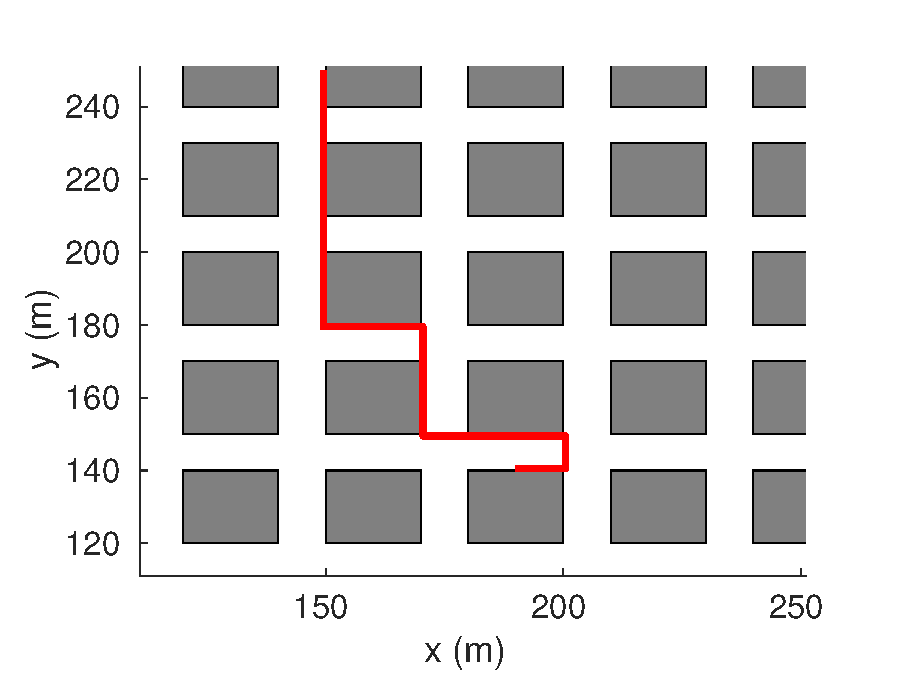
\includegraphics[width=2.25in]{./graphics/pedestrian_route.eps}%
 \label{fig_pedestrian_route}}
\hfil
\subfloat[Vehicular]{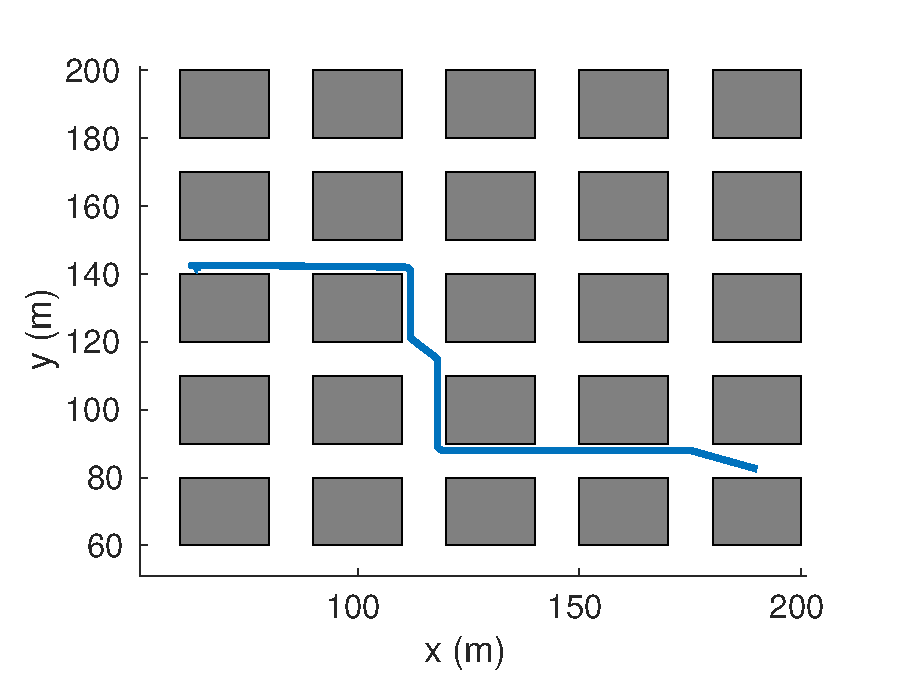
\includegraphics[width=2.25in]{./graphics/vehicular_route.eps}%
\label{fig_vehicular_route}}
\caption{Examples of trajectories for the two mobility models.}
\label{fig:routes}
\end{figure*}

The two learning methods were trained on the same RSSI data, generated by simulating a realistic urban scenario. The wireless channel we considered used a $945$ MHz downlink carrier frequency (one of the commercial bands used in LTE), and the users moved in a Manhattan grid of 100 buildings.

The grid we used is composed of 20 m wide square buildings, with 10 m wide one-way streets at each corner. The BS is placed at coordinates $(140,140)$, on top of a building close to the center of the simulation area.

\subsection{Propagation loss and fading}

The propagation loss was computed with the open-source system-level network simulator ns--3~\cite{ns3}. In particular, we used the LTE module~\cite{lena} and a radio propagation model called Hybrid Buildings Propagation Loss Model, which chooses the correct propagation model based on the reciprocal position of transmitter and receiver (both outdoors, both indoors, only one indoors). This model also takes into account the external wall penetration loss (for different types of buildings, i.e., concrete with windows, concrete without windows, stone blocks, wood), and the internal wall penetration loss.

We used the ns--3 simulation to create a square grid of path loss measures in our urban scenario, with a sampling distance of 33 cm. The path loss was then approximated as a linear combination of the 4 closest points in the grid, weighted by the relative distance. The main parameters of the ns--3 simulation are listed in Table~\ref{table:param}.

\begin{table}[!b]
\centering

\caption{Path loss computation parameters} % \usepackage{caption} if you want the caption below the table
\label{table:param}

\begin{tabular}{c|c}

\toprule
Parameter 						&	Value 			\\
\midrule
Downlink carrier frequency 		& 945 MHz			\\
Uplink carrier frequency		& 900 MHz			\\
RB bandwidth					& 180 kHz			\\
Available bandwidth				&  25 RB 			\\
eNB beamwidth					&  $360^{\circ}$ (isotropic)			\\
TX power used by eNBs 			&  43 dBm 			\\
eNB noise figure				&	3 dB 			\\
Number of buildings				&	100 				\\
Floors for each building		&	5 				\\
Radio Environment Map resolution & 9 samples/m\textsuperscript{2} \\
\bottomrule

\end{tabular}

\end{table}

The fading and shadowing processes were both generated in MATLAB, implementing well-known models. We used the log-normal model for shadowing, with a standard deviation of 4 dB and a correlation distance of 8 m.

Doppler fading was modeled with a Rayleigh distribution, using the parameters listed in Annex B.2 of \cite{lte136evolved} and the MATLAB Welch periodogram method. In the fading calculation, the node speed was assumed to be constant, simplifying the computation significantly with negligible error.

\subsection{Mobility model}
\label{sec:mobility}

We used two mobility models: \emph{pedestrian} and \emph{vehicular}. In both models, the user goes from point A to point B by choosing the direction that takes them closer to point B at each intersection.

In the \emph{pedestrian} model, a person walks at a constant speed of $1.5$ m/s along the side of the nearest building at a distance of $0.5$ m. Road crossings are placed at each intersection, and the pedestrian waits for a random time between 0 and 5 seconds before crossing to wait for cars.

In the \emph{vehicular} model, the driver keeps a constant speed of $15$ m/s while driving straight, switching between the 3 lanes by moving at a $45$ degree angle. Before a turn, the driver switches to the correct lane (e.g., they switch to the right lane before turning right), then slows down to $5$ m/s with a constant deceleration in the $5$ meters before the curve and makes a circular turn. After reaching the destination, the driver stops and reverses to slowly park on the curb, with a semi-circular trajectory.

The channel data was generated by running the urban scenario 5000 times for the pedestrian model and 10000 for the vehicular model, obtaining 3-4 days of data for the vehicular model and 20 hours for the pedestrian model (the car reaches its destination faster, so the traces are shorter). Two example trajectories for both models are shown in Fig.~\ref{fig:routes}.

\subsection{Learning parameters and results}

Both prediction methods were trained on the full dataset, with two different sampling rates: the channel was averaged over a window of 1 s and 0.5 s.

\begin{figure}[ht]
\centering
\includegraphics[width=3in]{./graphics/pedestrian_1s.eps}
\caption{Prediction error for the pedestrian scenario (1 s window).}
\label{pedestrian1s}
\end{figure}

\begin{figure}[t]
\centering
\includegraphics[width=3in]{./graphics/vehicular_1s.eps}
\caption{Prediction error for the vehicular scenario (1 s window).}
\label{vehicular1s}
\end{figure}

The Bayesian model used a Gaussian prior, centered on the last known channel sample; the probability vector for all classes was multiplied by a factor $k$ to obtain the Dirichlet parameter vector $\alpha$. Both the prior weight factor $k$ and the variance $\sigma$ of the Gaussian distribution were optimized as hyperparameters by cross-validation. The channel quantization step used to divide the data into classes was 2 dB.

As regards the SVR learning algorithm, we found the Radial Basis Function (RBF) kernel: $k(\mathbf z_i, \mathbf z_j ) = e^{- \gamma ||\mathbf z_i - \mathbf z_j||^2}$ to perform best with respect to other possible kernel choices. In this case, the hyperparameters of the model are $\gamma$ and $C$ in \eqref{eq:SVR_secondCost}: a  grid search on $(\gamma, C)$ pairs was thus performed, and the one with the best cross-validation RMSE was selected.

\begin{figure}[t]
\centering
\includegraphics[width=3in]{./graphics/pedestrian_05s.eps}
\caption{Prediction error for the pedestrian scenario (0.5 s window).}
\label{pedestrian05s}
\end{figure}

\begin{figure}[t]
\centering
\includegraphics[width=3in]{./graphics/vehicular_05s.eps}
\caption{Prediction error for the vehicular scenario (0.5 s window).}
\label{vehicular05s}
\end{figure}



After cross-validation, the performance of both prediction methods was measured on a previously unknown test set.

Fig.~\ref{pedestrian1s} shows the prediction RMSE for the pedestrian mobility model; the quality of the prediction is very good even with the simpler model, as pedestrians are slow and generally highly predictable. As expected, SVR clearly outperforms the naive Bayesian model, as it is able to generalize its experience and to better capture the features of the model. The gain of the longer memory is less pronounced for the Bayesian model, as it is overshadowed by the small size of the dataset (a longer memory means that a bigger dataset is necessary, and the memory-3 Bayesian model is not plotted, as its performance is not better than that with memory 2).



In the vehicular scenario, the RMSE is higher and the performance gap between the two methods is smaller (see Fig.~\ref{vehicular1s}); the Bayesian model even outperforms the SVR if the prediction is more than 3 seconds ahead, but a prediction error of more than 7 dB is only slightly better than no prediction at all (the prediction RMSE when using a memoryless channel model is about 8 dB). This may be due to the high speed of the vehicles ($\sim10$ times the speed of the pedestrians), which makes accurate generalizations about the evolution of the channel hard.

Fig.~\ref{pedestrian05s} and Fig.~\ref{vehicular05s} show the performance of the Bayesian method with a channel sampling window of 0.5 s; due to the computational cost of the SVR training, its performance in this case has not been evaluated.
The figures show that the trend in the performance of the Bayesian method is essentially the same, although the error is higher; the performance of the memory-3 Bayesian model shows that a longer memory is beneficial for the pedestrian model, but loses most of its benefits in the more chaotic vehicular scenario unless a bigger dataset is used.

Finally, Fig.~\ref{vehicularlowdata} shows the performance of the two predictors when they are trained with a reduced dataset: the two predictors were trained on 20\% of the available data in the vehicular scenario with a 1 second step. The plot shows how the performance of the SVR degrades far less than that with the Bayesian model, thanks to the former's ability to generalize experience. In fact, the reduced-dataset SVR performs better than the full-dataset Bayesian model when the prediction distance is less than 5 seconds.

\begin{figure}[t]
\centering
\includegraphics[width=3in]{./graphics/lowdata_vehicular_1s.eps}
\caption{Prediction error for the vehicular scenario (1 s window) including results using a reduced dataset.}
\label{vehicularlowdata}
\end{figure}

\section{Conclusions}

In this paper, we described and tested two learning-based methods to use past wireless channel information to predict the future channel gain. We compared the performance of the two methods over a synthetically generated dataset with random mobility for both pedestrian and vehicular scenarios.

The training was performed with just a few hours of RSSI data, so a BS with multiple connected users might be able to quickly gather the necessary training data and achieve a high-quality prediction in a very short time. However, the computational cost of the training itself is not negligible; while SVRs show a clear performance gain in both scenarios, the Bayesian model might be enough for applications that need a lower precision. It is worth noting that the SVR can have a satisfactory performance even when trained using a reduced dataset, as shown in Fig.~\ref{vehicularlowdata}; this makes it ideal if the limiting factor is not computational capability, but the size of the available dataset (e.g., in adaptive systems that are trained online to follow a time-varying scenario).
The quality of the predictions is generally high, and the RMSE is almost as low as the results shown in \cite{liao2015channel}, but without the use of GPS data, thereby reducing the energy consumption.

Future work may include a refinement of the prediction methods and the training of the predictors on data from real cellular systems.
Finally, a promising development might include the creation of a prediction-based resource optimization system like the one presented in \cite{mekki2015anticipatory}.

% An example of a floating figure using the graphicx package.
% Note that \label must occur AFTER (or within) \caption.
% For figures, \caption should occur after the \includegraphics.
% Note that IEEEtran v1.7 and later has special internal code that
% is designed to preserve the operation of \label within \caption
% even when the captionsoff option is in effect. However, because
% of issues like this, it may be the safest practice to put all your
% \label just after \caption rather than within \caption{}.
%
% Reminder: the "draftcls" or "draftclsnofoot", not "draft", class
% option should be used if it is desired that the figures are to be
% displayed while in draft mode.
%
%\begin{figure}[!t]
%\centering
%\includegraphics[width=2.5in]{myfigure}
% where an .eps filename suffix will be assumed under latex, 
% and a .pdf suffix will be assumed for pdflatex; or what has been declared
% via \DeclareGraphicsExtensions.
%\caption{Simulation results for the network.}
%\label{fig_sim}
%\end{figure}

% Note that the IEEE typically puts floats only at the top, even when this
% results in a large percentage of a column being occupied by floats.


% An example of a double column floating figure using two subfigures.
% (The subfig.sty package must be loaded for this to work.)
% The subfigure \label commands are set within each subfloat command,
% and the \label for the overall figure must come after \caption.
% \hfil is used as a separator to get equal spacing.
% Watch out that the combined width of all the subfigures on a 
% line do not exceed the text width or a line break will occur.
%
%\begin{figure*}[!t]
%\centering
%\subfloat[Case I]{\includegraphics[width=2.5in]{box}%
%\label{fig_first_case}}
%\hfil
%\subfloat[Case II]{\includegraphics[width=2.5in]{box}%
%\label{fig_second_case}}
%\caption{Simulation results for the network.}
%\label{fig_sim}
%\end{figure*}
%
% Note that often IEEE papers with subfigures do not employ subfigure
% captions (using the optional argument to \subfloat[]), but instead will
% reference/describe all of them (a), (b), etc., within the main caption.
% Be aware that for subfig.sty to generate the (a), (b), etc., subfigure
% labels, the optional argument to \subfloat must be present. If a
% subcaption is not desired, just leave its contents blank,
% e.g., \subfloat[].


% An example of a floating table. Note that, for IEEE style tables, the
% \caption command should come BEFORE the table and, given that table
% captions serve much like titles, are usually capitalized except for words
% such as a, an, and, as, at, but, by, for, in, nor, of, on, or, the, to
% and up, which are usually not capitalized unless they are the first or
% last word of the caption. Table text will default to \footnotesize as
% the IEEE normally uses this smaller font for tables.
% The \label must come after \caption as always.
%
%\begin{table}[!t]
%% increase table row spacing, adjust to taste
%\renewcommand{\arraystretch}{1.3}
% if using array.sty, it might be a good idea to tweak the value of
% \extrarowheight as needed to properly center the text within the cells
%\caption{An Example of a Table}
%\label{table_example}
%\centering
%% Some packages, such as MDW tools, offer better commands for making tables
%% than the plain LaTeX2e tabular which is used here.
%\begin{tabular}{|c||c|}
%\hline
%One & Two\\
%\hline
%Three & Four\\
%\hline
%\end{tabular}
%\end{table}


% Note that the IEEE does not put floats in the very first column
% - or typically anywhere on the first page for that matter. Also,
% in-text middle ("here") positioning is typically not used, but it
% is allowed and encouraged for Computer Society conferences (but
% not Computer Society journals). Most IEEE journals/conferences use
% top floats exclusively. 
% Note that, LaTeX2e, unlike IEEE journals/conferences, places
% footnotes above bottom floats. This can be corrected via the
% \fnbelowfloat command of the stfloats package.

% conference papers do not normally have an appendix

% trigger a \newpage just before the given reference
% number - used to balance the columns on the last page
% adjust value as needed - may need to be readjusted if
% the document is modified later
%\IEEEtriggeratref{11}
% The "triggered" command can be changed if desired:
%\IEEEtriggercmd{\enlargethispage{-5in}}

% references section

% can use a bibliography generated by BibTeX as a .bbl file
% BibTeX documentation can be easily obtained at:
% http://mirror.ctan.org/biblio/bibtex/contrib/doc/
% The IEEEtran BibTeX style support page is at:
% http://www.michaelshell.org/tex/ieeetran/bibtex/
\bibliographystyle{IEEEtran}
% argument is your BibTeX string definitions and bibliography database(s)
\bibliography{IEEEabrv,./IEEEabrv.bib}
%


% that's all folks
\end{document}


